\documentclass[12pt]{article}
\usepackage{scicite}
\usepackage{url}
\usepackage{times}
\usepackage{xcolor}
\usepackage{graphicx}
\usepackage{listings}


\topmargin 0.0cm
\oddsidemargin 0.2cm
\textwidth 16cm 
\textheight 21cm
\footskip 1.0cm

\renewcommand\refname{References and Notes}

\graphicspath{ {./assets/} }


\newcounter{lastnote}
\newenvironment{scilastnote}{%
\setcounter{lastnote}{\value{enumiv}}% 
\addtocounter{lastnote}{+1}%
\begin{list}%
{\arabic{lastnote}.}
{\setlength{\leftmargin}{.22in}}
{\setlength{\labelsep}{.5em}}}
{\end{list}}

\title{Investigation of an Application and a specific spam email.} 


% Place the author information here.  Please hand-code the contact
% information and notecalls; do *not* use \footnote commands.  Let the
% author contact information appear immediately below the author names
% as shown.  We would also prefer that you don't change the type-size
% settings shown here.

\author
{Marco Maurer \\
Julian Stampfli\\
\\
\normalsize{Department of Information Technology, Berner Fachhochschule}\\
}

\date{\today}

%%%%%%%%%%%%%%%%% END OF PREAMBLE %%%%%%%%%%%%%%%%



\begin{document} 

% Double-space the manuscript.

\baselineskip24pt

% Make the title.

\maketitle 


% In setting up this template for *Science* papers, we've used both
% the \section* command and the \paragraph* command for topical
% divisions.  Which you use will of course depend on the type of paper
% you're writing.  Review Articles tend to have displayed headings, for
% which \section* is more appropriate; Research Articles, when they have
% formal topical divisions at all, tend to signal them with bold text
% that runs into the paragraph, for which \paragraph* is the right
% choice.  Either way, use the asterisk (*) modifier, as shown, to
% suppress numbering.

\clearpage


\section{A closer look into the network traffic of the Battle.net client}

Blizzard is a game developer company that created games like World of Warcraft, Starcraft, Diablo, and Hearthstone. As most of those are online multiplayer games, they have to be updated frequently. To manage that Blizzard released a game client called battle.net. The battle.net client manages the games, where they are stored on the local computer and how to keep them updated. It also gives a single-sign-on utility which is just convenience for the player that he doesn't need to log into every game. It has a social function too, but this is ignored in this paper. As a reference a screenshot is available in Figure \ref{fig:client}  \cite{battlenet}

\begin{figure}[h]
  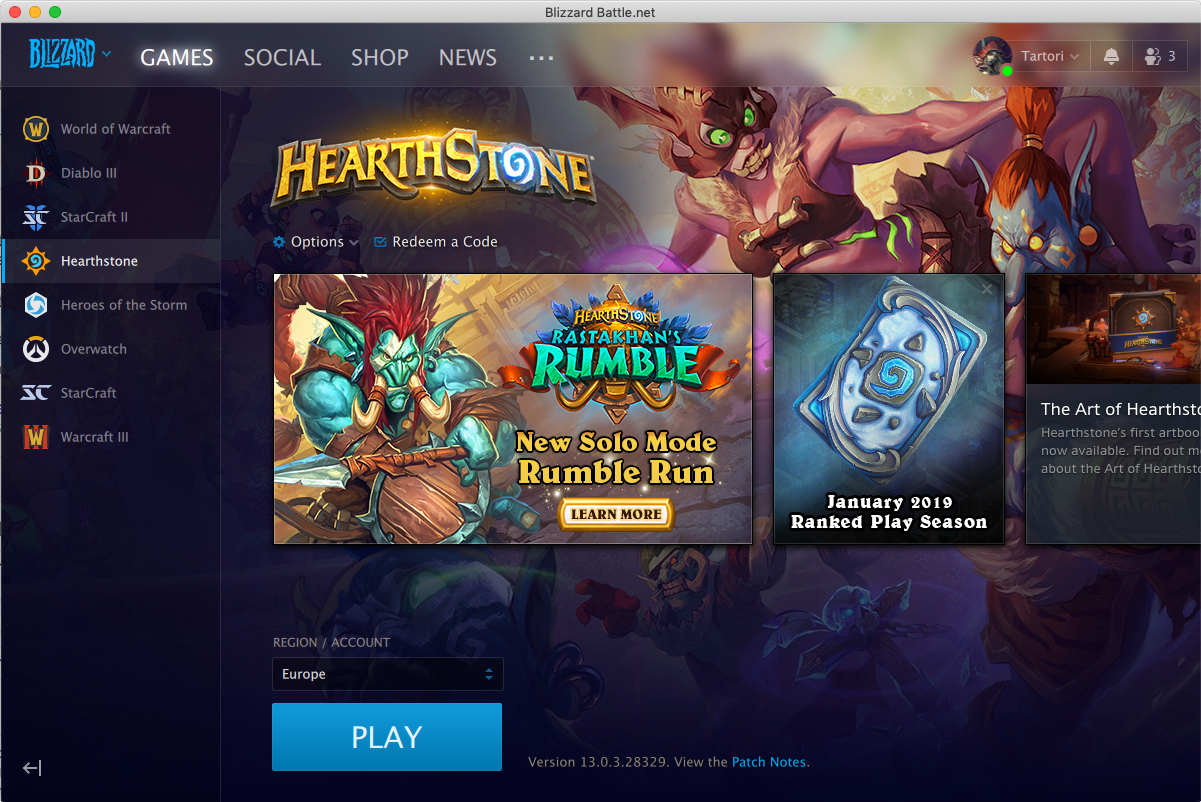
\includegraphics[width=8cm]{battlenetclient.png}
  \centering
  \caption{Battle.net client}
  \label{fig:client}
\end{figure}

\subsection{Methods}

To gather information about the battle.net client, there were several tools used. The test was run on a MacBook Pro with macOS Mojave version 10.14.2. To intercept the calls from the battle.net client proxifier was used to proxy only calls from the client and the Burp Suite community edition was used to intercept the traffic. The Burp Suite also did https interception, which is vital for this. LittleSnitch is used for the second part of the tests.

\subsection{Results and Discussion}

When running the setup as above, proxifier configured to proxy Battle.net to the Burp Suite it is apparently pretty fast that most calls are calls to the local machine. Most calls are actually to this process. There is an application called Agent.app running on the local machine as well. Including this one in the proxifier results in better results. Most of those results that call this agent look the same and can be viewed in section \ref{sec:agent_request}. 

These specific messages go through every few seconds. More messages call the agent service, but they are mostly about the configuration of the games. Thus the agent is most likely in charge of keeping the games up to date, informing the battle.net client about where they are stored. On startup of the client, it requests the /agent endpoint and receives an authorization response which it then uses on subsequent calls. This authorization is unique for each restart. On close, the client just calls the same endpoint, with the authorization and the DELETE verb. 

Aside from the agent calls which are very frequent, the application calls a host called telemetry-in.battle.net about every 30 seconds. These calls are some keep-alive. What for exactly is not clear. An example of this request is available in section \ref{sec:telemetry}

The client doesn't do much else when idle. More exciting things happen when it gets requests by changing views. It acts like a web browser and loads all the data at request. This behavior is not surprising as it reduces overhead. The data gets loaded from cache-eu.battle.net which sounds all right. For some game tabs, more information is loaded that is game specific. For instance, in Hearthstone the client checks if there is a fireside gathering nearby, which is a social gathering of players. 

Most of the calls of the battle.net client explained so far are to domains that are controlled by blizzard. It is to be expected that a client that displays information frequently needs to connect to the internet to get all the information. Aside from those calls the battle.net client also has requested the google-analytics endpoint. It sends a request there whenever the user changes the view. Those requests are made stealthy as the request directly goes to an IP and not to a DNS name. This request can be viewed in \ref{sec:google_analytics}

That this google-analytics works properly it also regularly asks whether the analytics.js has been updated. This call can be seen in \ref{sec:google_analytics_js}. 

When the proxy settings are disabled little snitch can display a map of all the connections of any specific application. The battle.net and agent application mostly communicate with servers in Europe and the US. The calls to the US are not surprising as blizzard is a US-based company. Many calls are residing in Switzerland. This behavior is reasonable as blizzard has a big network of servers to keep their latency low. The network traffic per country can be viewed in Figure \ref{fig:network}.

\begin{figure}[h]
  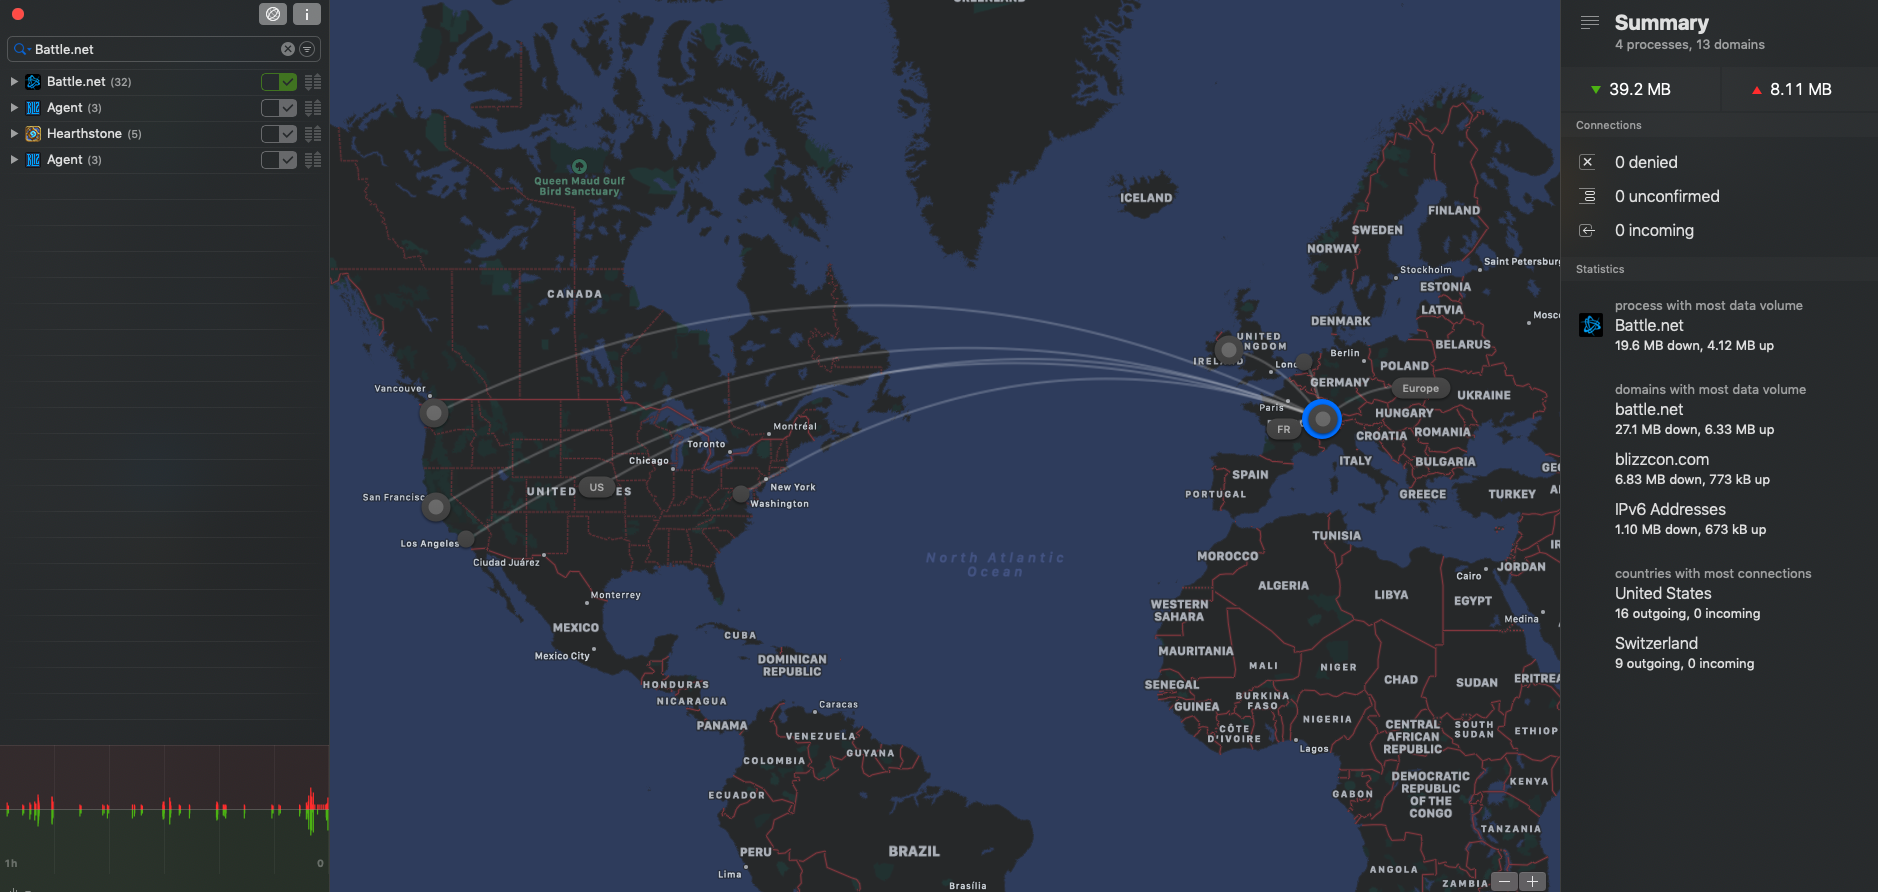
\includegraphics[width=12cm]{networkmonitor.png}
  \centering
  \caption{Little Snitch Network Monitor for Battle.net}
  \label{fig:network}
\end{figure}

\subsection{Conclusion}

Most of the calls the battle.net client does are necessary for its functionality. It needs to load the data on request, and the regular keep-alive is supposedly to update the online badge from the chat. The calls to google-analytics are unnecessary and can be disabled in a tool like little snitch.

Sadly we couldn't observe the traffic of the games themselves. They have certificate pinning which disables any attempt of SSL-interception. Based on the little snitch information Hearthstone for example only connects directly to servers and blizzard addresses. It also calls unity3d.com which is probably used because it was written in unity. 

\subsection{Requests}
\subsubsection{Agent}
\label{sec:agent_request}

Request:
\begin{lstlisting}
GET /gamesession HTTP/1.1
Host: 127.0.0.1:1120
User-Agent: phoenix-agent/1.0
Accept: */*
Authorization: 2351E52FD1FF53BD79C143BCAE3B8803
pid: 3808
Connection: close
\end{lstlisting}
Response:
\begin{lstlisting}
HTTP/1.0 200 OK
Content-Length: 737

{
  "hs_beta" : {
    "1" : {
      "request_id" : 4271.000000,
      "pid" : -1.000000,
      "pid_path" : "/Applications/Hearthstone/Hearthstone.app
      /Contents/MacOS/Hearthstone",
      "binary_type" : "game"
    },
    "2" : {
      "request_id" : 4276.000000,
      "pid" : -1.000000,
      "pid_path" : "/Applications/Hearthstone/Hearthstone.app
      /Contents/MacOS/Hearthstone",
      "binary_type" : "game"
    }
  },
  "battle.net" : {
    "1" : {
      "request_id" : 0.000000,
      "pid" : -1.000000,
      "pid_path" : "/Applications/Battle.net.app
      /Contents/MacOS/Battle.net",
      "binary_type" : "game"
    },
    "2" : {
      "request_id" : 0.000000,
      "pid" : 3808.000000,
      "pid_path" : "/Applications/Battle.net.app
      /Contents/MacOS/Battle.net",
      "binary_type" : "game"
    }
  }
}
\end{lstlisting}

\subsubsection{Telemetry}
\label{sec:telemetry}

Request:
\begin{lstlisting}
  POST /data HTTP/1.1
  Host: telemetry-in.battle.net
  Accept: */*
  Content-Type: application/octet-stream
  Pragma: no-cache
  Date: Sun, 13 Jan 2019 07:11:05 UTC
  Connection: close
  Content-Length: 246
  User-Agent: Agent/2.16.2.6563 cpp/3.1.6 Darwin/18.2.0
  Cache-Control: no-cache
  Content-Type: application/octet-stream
  
  
  ?
  1
  distAgent
           2.16.2.6563?
  cpp3.1.????-?M
  $954046F6-3866-4EFE-A8CD-215A7CE33ADBclient*macRx86_64?
  Darwin?18.2.028606311393901484513%
  Blizzard.Telemetry.Distribution.AgentRibbitWatchdog"
  eu.version.battle.net
\end{lstlisting}
Response:
\begin{lstlisting}
  HTTP/1.1 202 Accepted
  Content-Length: 0
  Date: Sun, 13 Jan 2019 07:21:36 GMT
  Connection: keep-alive  
\end{lstlisting}

\subsubsection{Google Analytics}
\label{sec:google_analytics}

Request:
\begin{lstlisting}
  POST /collect HTTP/1.1
  Host: www.google-analytics.com
  User-Agent: Battle.net/1.12.7.10892
  Accept: */*
  Content-Type: text/plain
  Content-Length: 233
  Connection: close
  v=1
  &tid=UA-50249600-2&cid=3BF72A96-A64B-4270-B803-72FA672DA6E1
  &z=9&an=APP&av=1.12.7.10892&ul=en-gb&uid=124383837
  &cd4=3BF72A96-A64B-4270-B803-72FA672DA6E1&cd1=1
  &cd3=0&cd2=1.12.7.10892&t=pageview&dh=EU.battle.net
  &dp=%2Fplay%2FS1_retail
\end{lstlisting}
Response:
\begin{lstlisting}
  Empty
\end{lstlisting}

\subsubsection{Google Analytics JS}
\label{sec:google_analytics_js}

Request:
\begin{lstlisting}
  GET /analytics.js HTTP/1.1
  Host: www.google-analytics.com
  Connection: close
  User-Agent: Mozilla/5.0 (Macintosh; 
  Intel Mac OS X 10_14_2) AppleWebKit/537.36 
  (KHTML, like Gecko) Battle.net/1.12.7.10892 
  Chrome/69.0.3497.81 Safari/537.36
  Accept: */*
  Referer: https://eu.battle.net/playscreen/html/
  eu/en-gb/?date=2017-05-30
  Accept-Encoding: gzip, deflate
  Accept-Language: en-GB,en;q=0.9
  If-Modified-Since: Mon, 05 Nov 2018 21:10:09 GMT

\end{lstlisting}
Response:
\begin{lstlisting}
  HTTP/1.1 304 Not Modified
  Date: Sat, 12 Jan 2019 17:25:58 GMT
  Expires: Sat, 12 Jan 2019 19:25:58 GMT
  Age: 1865
  Alt-Svc: quic=":443"; ma=2592000; v="44,43,39,35"
  Connection: close
\end{lstlisting}






\newpage


\section{A closer look into a spam email.}

\begin{figure}[h]
 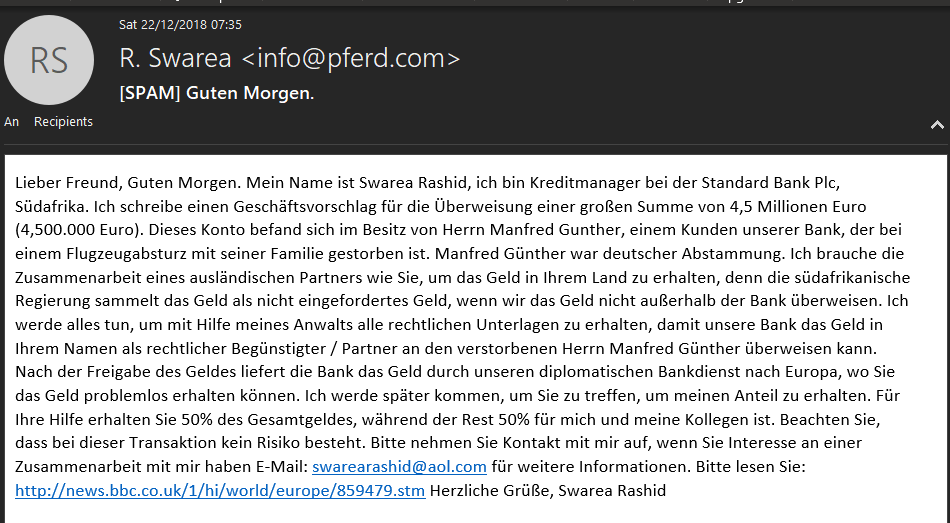
\includegraphics[width=15cm]{mail.png}
  \centering
  \caption{Spam mail}
  \label{fig:spam}
\end{figure}

In figure \ref{fig:spam} is the mail I'd like to analyze. I responded to it to see what precisely the sender wanted from me. So far, I received 3 more, but unfortunately, the communication is rather slow. That's why I can't tell exactly the intention behind this email. I think there's going to be a request for money at some point. Until now I had to give him my address. Otherwise, he gives the impression that everything is running according to plan. In his last mail, he said that I have to travel to Amsterdam to receive the money.

\subsection{Truth content}
\subsubsection{First mail}
\begin{enumerate}
\item the bank\\
Mr. Swarea indicates to work for the Standard Bank PLC. This bank exists. It’s a big bank in South Africa. However, the ending PLC is wrong. Only the London branch of the bank has this extension. In South Africa PLC is not a common extension for a company.
\item the person\\
The mail refers to the crash of the Concorde in Paris. Unfortunately, I couldn’t find out if Mr. Günther was sitting in this plan or not. However, since all passenger on board were German, it could be possible. However, since the accident happened in 2000, it is doubtful that the money is still on the bank.
\end{enumerate}

\subsubsection{Second and third mail}
There's nothing to analyze in these emails. He said that he is communicating with his lawyer and that it would take a little longer.

\subsubsection{Fourth mail}
He sent me an e-mail with different confirmation from his lawyer. He also says that the courier cannot travel to Switzerland because he has no diplomatic immunity. That' s why I have to travel to Amsterdam to get the money.  The story has two problems:

\begin{enumerate}
\item Why should a diplomat not have immunity in Switzerland and why is that even necessary?
\item One recognizes immediately that all documents are forged. The sender does not even try to give the impression that the documents are real. As a reference to that in figure \ref{fig:seal} is an actual seal of the South African government.
\end{enumerate}

\begin{figure}[h]
 
\includegraphics[width=8cm]{seal.png}
  \centering
  \caption{How the seal of the South African government should look like}
  \label{fig:seal}
\end{figure}

\subsection{Addresses}
The domain pferd.com belongs to a German company that manufactures tools. The SPF Policy of the company marked the mail as soft fail. That's why the mail was marked as spam by my email provider.  The IP address (188.206.70.138) of the sender is located in the Netherlands. The reply address is swarearashid@aol.com (IP Address: 74.6.134.42). Unfortunately, I could only trace this address back to the server of yahoo. This server is located in Sunnyvale California.
I did the header analysis with www.gaijin.at \cite{mailHeader} and for the IP lookup, I used www.iplocation.net \cite{iploc}.

\subsection{HTML}
The analysis of the HTML code is not very interesting. It is a pure text message. Therefore, there is nothing special to be found. 

\subsection{Link}
The link http://news.bbc.co.uk/1/hi/world/europe/859479.stm  leads to an article about the Concorde crash on the BBC website. It is only used to convince the recipient that Mr. Günther died in a plane crash. There is no phishing and no JavaScript in the background. 

\subsection{Where does he get my mail address?}
My father received this mail on his business e-mail address. This address is easy to find on the internet. I think the address also appears on various address lists. Which you can buy everywhere. For Switzerland, you can buy a list with 170’000 business addresses for 200 Euro \cite{adresspool}.

\subsection{Sender}
I think the person is sending the emails for fun or boredom. If he wanted to earn money with it, he would spend more time on it. The documents he sent me could certainly be made more authentic with a little more effort. She doesn't have to be technically gifted. For this kind of spam basic computer knowledge is enough. Everything he needs can be found on Google without any problem.


\clearpage

\bibliography{privacy}

\bibliographystyle{Science}



\end{document}
